\documentclass[11pt,a4paper]{article}

\usepackage[T1]{fontenc}
\usepackage[utf8]{inputenc}
\usepackage{lmodern}
\usepackage{microtype}
\usepackage{geometry}
\geometry{margin=24mm}
\setlength{\emergencystretch}{3em}

\usepackage{amsmath,amssymb,amsthm,mathtools}
\usepackage{booktabs}
\usepackage{array}
\usepackage{longtable}
\usepackage{tabularx}
\usepackage{enumitem}
\usepackage{xurl}
\usepackage{xspace}
\usepackage{graphicx}
\usepackage{tikz}
\usetikzlibrary{arrows.meta,positioning,fit,calc,shapes.geometric}
\usepackage[hidelinks]{hyperref}
\hypersetup{
  pdftitle={Split Complex Lorentzian Dynamics - Part XXXI: Exact Kernel-Defect Classification, Explicit Nontriviality, and the Atlas-Dependence Frontier},
  pdfauthor={Jan Seeck; OpenAI ChatGPT; Aristotle (Harmonic)},
  pdfsubject={Task-31 fixed-presentation liftability classification, explicit neutral and non-neutral systems, and the ordinary-atlas dependence revealed by source review},
  pdfkeywords={split-complex Lorentz structure, internal lift, kernel defect, frame atlas, transition system, spin frontier, local trivialization, Lean, formal verification, conservation of difficulty}
}
\usepackage[nameinlink,noabbrev]{cleveref}
\usepackage{csquotes}
\usepackage[backend=biber,style=numeric,sorting=nyt,maxbibnames=20]{biblatex}
\AtBeginBibliography{\scriptsize\raggedright}
\addbibresource{Split_Complex_Lorentzian_Dynamics_Part_XXXI_references.bib}

\newtheorem{theorem}{Theorem}
\newtheorem{proposition}{Proposition}
\newtheorem{corollary}{Corollary}
\newtheorem{remark}{Remark}
\newtheorem{boundary}{Proof boundary}
\newtheorem{question}{Open question}
\newtheorem{caveat}{Methodological caveat}
\theoremstyle{definition}
\newtheorem{definition}{Definition}
\newtheorem{status}{Status}
\newtheorem{principle}{Methodological principle}
\newtheorem{reviewfinding}{Review finding}

\newcommand{\R}{\mathbb{R}}
\newcommand{\Ztwo}{\{\pm1\}}
\newcommand{\Lift}{\mathcal{L}}
\newcommand{\Gvis}{G_{\mathrm{vis}}}
\newcommand{\Ker}{K}
\newcommand{\proj}{p}
\newcommand{\ITot}{\mathcal{I}}
\newcommand{\FTot}{\mathcal{F}^{+}}
\newcommand{\Def}{\mathfrak{D}}
\newcommand{\code}[1]{\path{#1}}
\newcommand{\Lean}{\textsc{Lean}\xspace}
\newcommand{\TaskThirty}{\textsc{Task 30}\xspace}
\newcommand{\TaskThirtyOne}{\textsc{Task 31}\xspace}
\newcommand{\TaskThirtyTwo}{\textsc{Task 32}\xspace}

\title{\textbf{Split Complex Lorentzian Dynamics}\\[0.45em]
\large Part XXXI: Exact Kernel-Defect Classification, Explicit Nontriviality, and the Atlas-Dependence Frontier\\[0.35em]
\normalsize From fixed-presentation existence to the discovery that the ordinary frame atlas itself remains above the intrinsic geometric level}

\author{%
\textbf{Editor:} Jan Seeck\\
\textbf{AI Assistant:} OpenAI ChatGPT (GPT-5.6 Sol)\\
\textbf{Lean Agent:} Aristotle (Harmonic)}
\date{6 September 2026}

\begin{document}
\maketitle

\begin{abstract}
Part~XXX ended at a deliberately dramatic boundary.  Once continuous internal transition maps
\[
 u_{ij}:U_i\cap U_j\longrightarrow\Lift
\]
with
\[
 \proj(u_{ij})=g_{ij},\qquad u_{ii}=1,\qquad u_{ji}=u_{ij}^{-1},\qquad u_{jk}u_{ij}=u_{ik}
\]
were assumed, every remaining construction step closed: the local products glued to a genuine topological total space, the globally descending right $\Lift$-action was continuous and fibrewise free and transitive, and the global map to the ordinary oriented-frame total space had fibres exactly equal to kernel orbits.  The only principal arrow left open was existence of the compatible transition system itself \cite{Experiment2PartXXX2026,AristotleTask30_2026}.

Task~31 attacks that arrow and obtains a substantial formal closure at the level of a \emph{fixed ordinary transition system}.  First, the small Task-30 interface gap is closed: the global map
\[
 \Pi:\ITot\longrightarrow\FTot
\]
is proved surjective; every ordinary frame therefore has an upstairs fibre; every such fibre is a free transitive $\Ker(\proj)$-set; and for the certified two-element kernel every fibre has cardinality two.  In the inherited chart models, a local product homeomorphism of the form ``visible neighborhood $\times$ kernel'' is constructed around every point.  The Mathlib predicate \code{IsCoveringMap} is not packaged, but the explicit local two-sheeted model is proved.

The task then freezes
\[
 \operatorname{InternalLiftable}(S)
 \;:\Longleftrightarrow\;
 \operatorname{Nonempty}(\operatorname{CompatibleContinuousInternalTransitions}(S))
\]
and reconstructs a quotient-valued kernel-defect state for each internal candidate.  If $\delta_{ijk}$ denotes the inherited kernel-valued triple defect, admissible kernel adjustments $\varepsilon_{ij}$ act by
\[
 \delta'_{ijk}
 = (\varepsilon_{jk}\varepsilon_{ij}\varepsilon_{ik}^{-1})\,\delta_{ijk}.
\]
The corresponding equivalence relation is proved reflexive, symmetric and transitive and is quotiented.  Because different refined candidates live on different defect domains, the complete quotient classes are not silently identified across candidates.  What \emph{is} proved candidate-, kernel-gauge-, and Task-XXVIII-refinement-independent is the statement that the defect class is neutral.  Task~31 then proves its central theorem:
\[
 \boxed{
 \operatorname{InternalLiftable}(S)
 \iff
 \operatorname{IsNeutralGlobalKernelDefect}(S).}
\]
Thus, for a fixed ordinary transition system, the previously isolated simultaneous kernel equations have become an exact necessary-and-sufficient existence criterion.

Universal direct liftability of such fixed systems is formally refuted.  Over the base $B=\Gvis$ and the two-chart cover $U_0=U_1=B$, Task~31 constructs a positive system with all transitions equal to $1$ and a negative system with
\[
 g_{00}=g_{11}=1,\qquad g_{01}(b)=b,\qquad g_{10}(b)=b^{-1}.
\]
The positive system is liftable and neutral.  A compatible lift of the negative system would make $u_{01}$ a continuous global section of the already certified projection $\Lift\to\Gvis$, contradicting the inherited no-global-representative theorem.  Hence the negative system is non-liftable and its defect state is non-neutral.  The supplied Lean layer therefore proves both a neutral and a non-neutral state and records formal verdict N: universal existence is refuted, with exact classification by neutrality \cite{AristotleTask31_2026}.

The source review, however, exposes a deeper boundary that is not captured by that formal verdict.  The negative transition system is additionally realized as a Task-XXVII topological frame family, but its underlying metric-oriented rank-three family is \emph{constant}.  Moreover, the source itself defines \code{badTriv0} on the whole base as the identity metric-oriented fibre trivialization.  A second global chart \code{badTriv1} is obtained by applying the base point $b\in\Gvis$ as a rotation, and precisely this redundant chart produces $g_{01}(b)=b$.  Consequently the same underlying constant family admits a globally trivial presentation whose transition system is neutral, while the selected two-chart presentation is not directly liftable on its whole overlaps.

This distinction changes the interpretation, not the correctness, of the Lean theorems.  Task~31 has proved that neutrality is intrinsic with respect to internal representative choices, kernel gauges and the \emph{candidate refinements of a fixed ordinary transition system}.  It has \emph{not} proved invariance under replacement of the ordinary frame atlas itself, under ordinary chart gauge changes, or under refinement/change of the ordinary cover.  Therefore the current non-neutral example is an exact counterexample to universal \emph{fixed-presentation} liftability, but it is not yet an atlas-independent counterexample to existence of a global spatial spin-like lift of the underlying frame geometry.

The Conservation-of-Difficulty principle therefore acts once again.  The obstruction has not disappeared, but neither has it reached bedrock.  Local representatives, repeated-index coherence, same-pair descent, simultaneous kernel equations, global gluing, surjectivity and exact two-sheeted fibres are no longer the frontier.  The remaining difficulty has moved one level deeper, into the quotient by ordinary presentation data itself:
\[
 \boxed{
 \text{internal kernel gauges}
 \;+
 \text{ordinary frame-chart changes}
 \;+
 \text{ordinary cover refinements}.}
\]
Part~XXXII should reconstruct that quotient intrinsically.  It must determine whether the neutral/non-neutral defect state descends from a fixed transition presentation to the underlying metric-oriented frame family, repair the present ``bad'' control under an atlas change, and then decide whether a genuinely atlas-independent non-neutral example survives.  Only after that step can the project legitimately claim either a global spatial lift obstruction or a spatial spin-structure closure.  The excavation therefore continues: Task~31 closes one equation system exactly and, in doing so, reveals that the ordinary atlas was still one floor above the desired invariant geometry.
\end{abstract}

\noindent\textbf{Keywords:} kernel defect; internal liftability; ordinary transition system; frame atlas; atlas dependence; local two-sheeted product; global gluing; fixed-presentation obstruction; formal verification; Lean~4; Conservation of Difficulty; spin frontier.

\tableofcontents
\newpage

\section{The promise inherited from Part XXX: one equation system from closure}\label{sec:promise}

Part~XXX had removed every construction ambiguity downstream of compatible internal transitions.  If a continuous family $u_{ij}$ satisfying the four compatibility laws existed, then the local products $U_i\times\Lift$ glued, the quotient topology was the intended local-product topology, the internal group acted globally on the right, and the visible projection had exact kernel fibres \cite{Experiment2PartXXX2026}.  The remaining chain was therefore
\begin{equation}\label{eq:part30chain}
\begin{aligned}
 \text{solve the kernel equations}
 &\Longleftrightarrow \text{compatible internal transitions exist}\\
 &\Longrightarrow \text{global internal object exists}.
\end{aligned}
\end{equation}

The temptation was obvious: Task~31 might be the first true global closure of the spatial branch.  The task was therefore deliberately written as a closure test rather than as another broad exploration.  It had to harden the global map, decide universal existence honestly, and, if universality failed, reconstruct the exact intrinsic datum that controlled fixed-system existence.

\begin{principle}[Closure must survive a change of level]
A theorem may close an existence question for a chosen presentation without yet closing the corresponding geometric existence question.  Whenever the formal carrier still includes chart, cover, representative or gauge choices as data, the next audit must test whether the claimed invariant descends through those choices.
\end{principle}

This principle is not an objection imported after the fact.  It is the same top-to-bottom methodology used throughout the reconstruction: once one variable has been solved in terms of deeper variables, one must inspect whether the latter are themselves derived presentation data.

\section{Formal source, verification boundary and provenance}\label{sec:formal}

The supplied Task-31 archive has SHA-256
\begin{center}
\code{aee5b476e5fc7880e5ac11dc9f7258795dae2e815d0d55a395fb9512928a5d29}.
\end{center}
The pinned environment is Lean~4.28.0 with Mathlib commit
\begin{center}
\code{8f9d9cff6bd728b17a24e163c9402775d9e6a365}.
\end{center}
The Task-XXVII, XXVIII, XXIX and XXX source directories were compared against the preceding Task-30 archive and are byte-for-byte unchanged.

Task~31 adds ten Lean files and 1848 Lean source lines:
\begin{center}
\small
\code{LiftabilityPredicate}
$\to$ \code{GlobalMapHardening}
$\to$ \code{UniversalExistenceAudit}
$\to$ \code{IntrinsicDefectState}
$\to$ \code{DefectNeutrality}
$\to$ \code{ExistenceClassification}
$\to$ \code{SpatialClosureInterface}
$\to$ \code{GlobalCoveringHardening}
$\to$ \code{FrameFamilyRealization}
$\to$ \code{Task31}.
\end{center}

\begin{longtable}{>{\raggedright\arraybackslash}p{0.34\textwidth}p{0.19\textwidth}p{0.37\textwidth}}
\toprule
Check & Result & Detail\\
\midrule
\endfirsthead
\toprule Check & Result & Detail\\
\midrule
\endhead
Focused Task-31 build & PASS & \code{lake build RequestProject.NullSectorTask31.Task31}\\
Whole-project build & PASS & 8350 jobs, exit code 0\\
Task-31 warnings & 0 & inherited warnings unchanged\\
New source & 10 Lean files & 1848 Lean lines\\
Axiom audit & 69 reports & only \code{propext}, \code{Classical.choice}, \code{Quot.sound}\\
Proof holes & 0 & no \code{sorry}, \code{admit}, custom axiom\\
Prohibited escapes & 0 & no \code{native_decide}, \code{bv_decide}, \code{implemented_by}, prohibited \code{unsafe} or \code{partial}\\
Preserved failed builds & 5 & all repaired without mathematical weakening\\
\bottomrule
\end{longtable}

\begin{boundary}[Verification boundary]
The supplied Task-31 source tree, audit, module chain, critical definitions, positive and negative examples, defect-class construction, global-map hardening, frame-family realization, endpoint statements, proof-escape scan and the relevant Task-29/30 inherited interfaces were inspected directly for this paper.  The successful focused and whole-project builds and the 69 \code{#print axioms} reports are reported from the supplied Aristotle artifact; the 8350-job project build was not independently rerun in the paper-generation environment.
\end{boundary}

The source audit itself records formal verdict N.  This paper accepts the Lean theorem statements at their proved level but subjects the \emph{interpretation} of that verdict to a further dependency audit.  That distinction is essential for the remainder of the paper.

\section{Hardening the global map: the conditional object really reaches every frame}\label{sec:surj}

Task~30 had proved a continuous equivariant map
\[
 \Pi:\ITot\to\FTot
\]
with exact kernel orbits over points in its image, but had not exposed global surjectivity as an endpoint.  Task~31 closes this gap.

The proof route is structurally minimal.  Given an ordinary frame $F\in\FTot$, choose an internal point $x\in\ITot$ over the same base point.  Fibrewise transitivity downstairs gives $g\in\Gvis$ carrying $\Pi(x)$ to $F$.  Surjectivity of $\proj:\Lift\to\Gvis$ gives $a\in\Lift$ with $\proj(a)=g$.  Equivariance then yields
\[
 \Pi(x\cdot a)=\Pi(x)\cdot\proj(a)=F.
\]
This is formalized as \code{GluedInternalFrameSystem.toFrame_surjective} and exposed again as \code{internalToFrame_surjective}.

\begin{theorem}[Global-map hardening, Task-31 level]
For every conditional Task-30 glued internal system, $\Pi$ is surjective onto all of $\FTot$.  Every ordinary frame has a nonempty upstairs fibre, and every such fibre is a free transitive $\Ker(\proj)$-set.  If $\operatorname{card}\Ker(\proj)=2$, every fibre has exactly two points.
\end{theorem}

Thus the set-level qualification ``over image points'' disappears.  The two-valued visible information loss is global over the entire ordinary frame total space whenever the conditional object exists.

\section{The local two-sheeted structure is also reconstructed}\label{sec:cover}

Task~31 further combines the inherited local sections of $\proj$, the Task-30 product charts upstairs and the Task-27 product charts downstairs.  The chart model of $\Pi$ is proved to be
\begin{equation}\label{eq:chartpi}
 (b,a)\longmapsto (b,\proj(a)\cdot f_{\mathrm{ref}}).
\end{equation}
On a visible neighborhood $V_G\subseteq\Gvis$ carrying a continuous local section $s:V_G\to\Lift$, the internal chart preimage is explicitly decomposed as
\begin{equation}\label{eq:localsheets}
 \text{topSet}\;\cong_{\mathrm{Top}}\;\text{botSet}\times\Ker(\proj).
\end{equation}
The second coordinate is exactly the residual kernel element
\[
 s(\proj(a))^{-1}a\in\Ker(\proj).
\]

An extra datum, \code{FrameModelSection}, is carried explicitly rather than smuggled into the abstract frame model.  It supplies a continuous inverse from the model-frame orbit back to the visible group.  Task~31 proves this datum for the inherited Task-27 model frame space.

\begin{status}[Covering boundary]
The explicit local two-sheeted product is proved in the inherited chart models around every ordinary chart point.  The statement \code{IsCoveringMap Pi} is not packaged, and the chart-model homeomorphism is not transported all the way to a global subspace homeomorphism $\Pi^{-1}(V)\cong V\times\Ker$ inside the glued total spaces.  Therefore ``two-sheeted local product'' is proved; ``Mathlib covering map'' remains a packaging/open-interface statement.
\end{status}

This is already sufficient for the main existence audit: the conditional object has the expected local two-sheeted geometry once it exists.

\section{Freezing the existence predicate}\label{sec:liftable}

Task~31 defines, for a fixed ordinary transition system $S$ and fixed internal projection $P$,
\begin{equation}\label{eq:liftable}
 \operatorname{InternalLiftable}(P,S)
 :\Longleftrightarrow
 \operatorname{Nonempty}\bigl(\operatorname{CompatibleContinuousInternalTransitions}(P,S)\bigr).
\end{equation}
For inherited ordinary systems the certified model projection is inserted, producing \code{OrdinaryInternalLiftable}.

Using Task~29, the new predicate is shown equivalent to simultaneous trivializability of the kernel defect equations.  More importantly, the Boolean existence predicate is proved independent of the chosen Task-XXVIII internal candidate, of kernel-valued representative gauges and of the specific candidate refinement operation inherited from Task~XXVIII/XXIX.

\begin{caveat}[What ``refinement'' means here]
The formal refinement theorem concerns \emph{candidate refinements} inside one fixed ordinary transition system.  The ordinary cover $U_i$ and the ordinary frame transition functions $g_{ij}$ remain fixed.  It is not yet a theorem about replacing the ordinary frame atlas by a refinement or by a different atlas of the same underlying metric-oriented family.
\end{caveat}

This caveat becomes decisive later.

\section{From the triple defect to a quotient-valued defect state}\label{sec:defectstate}

For an internal candidate $C$, Task~31 packages a continuous kernel-valued triple-overlap defect system.  The inherited representative-change law is retained exactly.  If $\varepsilon_{ij}$ is a kernel adjustment, then
\begin{equation}\label{eq:adjshift}
 \delta'_{ijk}
 =\bigl(\varepsilon_{jk}\varepsilon_{ij}\varepsilon_{ik}^{-1}\bigr)\delta_{ijk}.
\end{equation}
Task~31 defines \code{DefectEquivalent} by the existence of such an adjustment and proves reflexivity, symmetry and transitivity.  Therefore, for a fixed candidate $C$, one may form the quotient
\[
 \operatorname{DefectClass}(C)
 = \operatorname{DefectSystem}(C)/{\sim}.
\]
The actual defect and the everywhere-identity defect define two classes
\[
 [\delta_C],\qquad[1].
\]

\begin{definition}[Candidate-level neutral defect state]
A candidate $C$ is neutral if
\[
 [\delta_C]=[1]
\]
in its candidate-specific quotient type.
\end{definition}

The key local theorem is exact:
\begin{equation}\label{eq:candidate-neutral}
 C\text{ neutral}
 \iff
 C\text{ satisfies the Task-29 kernel equations}.
\end{equation}

The task correctly refuses to identify full quotient classes of different candidates: their refined defect domains may differ, so their quotient types differ.  Only the proposition of neutrality is transported across candidates.

\section{Neutrality becomes intrinsic relative to a fixed ordinary system}\label{sec:neutrality}

Task~31 defines
\begin{equation}\label{eq:globalneutral}
 \operatorname{IsNeutralGlobalKernelDefect}(P,S)
 :\Longleftrightarrow
 \forall C,\; C\text{ has neutral defect state}.
\end{equation}
It then proves that ``every candidate is neutral'' is equivalent to ``some candidate is neutral''.  Consequently a lucky or unlucky internal representative choice cannot change the answer.

The following invariances are formally established:
\begin{itemize}[leftmargin=*]
 \item internal representative choice does not affect neutrality;
 \item admissible kernel gauge does not affect neutrality;
 \item Task-XXVIII candidate refinement does not affect neutrality.
\end{itemize}

\begin{boundary}[Full defect-class canonicity]
The complete quotient class $[\delta_C]$ is canonical only relative to a candidate.  Task~31 does not construct a single quotient type into which the classes of all candidates or all refinements are transported.  The invariant exported across candidates is the Boolean proposition ``neutral or not''.  The Task-31 audit records this as PARTIAL for full class canonicity and PROVED for neutrality.
\end{boundary}

At this level the adjective ``intrinsic'' has a precise but limited meaning: intrinsic relative to the fixed ordinary system $S$ after quotienting the allowed \emph{internal} auxiliary choices.

\section{The central success theorem: fixed-system liftability iff neutrality}\label{sec:classification}

The main theorem of Task~31 is
\begin{theorem}[Exact fixed-system classification]\label{thm:classification}
For every fixed ordinary transition system $S$ and fixed internal projection $P$,
\begin{equation}\label{eq:classification}
 \boxed{
 \operatorname{InternalLiftable}(P,S)
 \iff
 \operatorname{IsNeutralGlobalKernelDefect}(P,S).}
\end{equation}
\end{theorem}

The proof is a clean consolidation of the previous tasks.  If compatible transitions exist, then Task~29 solves the kernel equations of every candidate, so every defect class is neutral.  Conversely, if one candidate is neutral, the quotient equality extracts an admissible kernel adjustment solving the Task-29 equations, and Task~29 returns compatible transitions on the original overlaps.

This is a genuine closure theorem.  No gluing question remains after neutrality: combining \cref{eq:classification} with Part~XXX and the Task-31 surjectivity hardening gives
\begin{equation}\label{eq:neutral-global}
 \text{neutral defect}
 \Longrightarrow
 \begin{cases}
 \text{global locally trivial }\ITot,\\
 \text{free/transitive right }\Lift\text{-action on base fibres},\\
 \Pi:\ITot\twoheadrightarrow\FTot\text{ continuous and equivariant},\\
 \Pi^{-1}(F)\text{ an exact }\Ker(\proj)\text{-torsor},\\
 |\Pi^{-1}(F)|=2\text{ in the certified instance}.
 \end{cases}
\end{equation}

The reverse implication from a global glued object is also proved at the exact strength inherited from Part~XXX: it requires \code{AdaptedCharts} so that the extracted internal transition functions are known to project to the already fixed ordinary transition presentation.

\section{Universal fixed-presentation liftability is refuted}\label{sec:universal}

Task~31 does not stop at the classification theorem.  It asks whether the inherited assumptions force neutrality for every ordinary transition system.  They do not.

Let
\[
 B=\Gvis,\qquad I=\{0,1\},\qquad U_0=U_1=B.
\]
Define
\begin{equation}\label{eq:badtrans}
 g_{00}=g_{11}=1,\qquad
 g_{01}(b)=b,\qquad
 g_{10}(b)=b^{-1}.
\end{equation}
Continuity, identity normalization, inverse symmetry and the triple-overlap law are proved directly.  Hence this is a legitimate inherited \code{OrdinaryTransitionSystem}.

Suppose compatible internal transitions existed.  Then the off-diagonal map $u_{01}$ would satisfy
\[
 \proj(u_{01}(b))=b
\]
continuously on all of $\Gvis$.  It would therefore be a continuous global representative of the identity map of the visible group.  The certified no-global-representative theorem from the earlier reconstruction refutes exactly this possibility \cite{AristotleTask23_2026,AristotleTask31_2026}.

\begin{theorem}[Negative fixed-presentation example]
The system \cref{eq:badtrans} is not internally liftable and has non-neutral global kernel defect in the sense of \cref{eq:globalneutral}.
\end{theorem}

Over the same base and same two-copy cover, Task~31 defines a positive control with every transition equal to $1$.  It is internally liftable and neutral.  Therefore
\begin{equation}\label{eq:nontrivial-state}
 \exists S_{+}:\operatorname{Neutral}(S_{+}),
 \qquad
 \exists S_{-}:\neg\operatorname{Neutral}(S_{-}).
\end{equation}
This is the formal theorem \code{globalKernelDefect_state_is_nontrivial} highlighted during the Task-31 run.

\section{The stronger realization: the negative system comes from an actual frame atlas}\label{sec:framefamily}

A possible objection to \cref{eq:badtrans} would be that it is merely an abstract transition system.  Task~31 therefore realizes it as an inherited Task-XXVII \code{TopologicalFrameFamily}.

The underlying family is defined explicitly as the constant metric-oriented rank-three family
\begin{equation}\label{eq:constant-family}
 E_b = \mathrm{Model}\qquad\text{for every }b\in\Gvis.
\end{equation}
It carries the same fixed model orientation in every fibre.

Two global trivializations are then defined on $B$ itself:
\begin{align}
 T_0(b) &= \operatorname{id}_{\mathrm{Model}},\label{eq:t0}\\
 T_1(b) &= b:\mathrm{Model}\to\mathrm{Model},\label{eq:t1}
\end{align}
where $b\in\Gvis$ is read as the reconstructed orientation-preserving metric linear isometry.  The overlap maps are proved continuous.  The transition from chart $0$ to chart $1$ is computed as
\begin{equation}\label{eq:family-transition}
 T_1(b)\,T_0(b)^{-1}=b.
\end{equation}
Thus the extracted ordinary transition system is exactly \cref{eq:badtrans}, and the formal non-liftability theorem is inherited by this atlas-equipped frame family.

At first glance, this looks like the strongest possible negative witness.  It is precisely here, however, that the next level of the dependency audit becomes visible.

\section{Review turning point: the ``bad'' family is globally trivial before the atlas is frozen}\label{sec:turning}

The source itself contains the decisive information.  The underlying family \cref{eq:constant-family} is constant, and $T_0$ in \cref{eq:t0} is already a global metric- and orientation-preserving trivialization on all of $B$.

\begin{reviewfinding}[The negative witness is presentation-sensitive]\label{rf:presentation}
The Task-31 theorem proves that the \emph{selected two-chart ordinary transition system} of \code{badFamily} is not directly liftable on its full overlaps.  It does not prove that the underlying constant metric-oriented rank-three family lacks a global internal lift independently of the chosen ordinary atlas.
\end{reviewfinding}

Indeed, if one presents the same constant family using only $T_0$, then the sole transition is
\[
 g_{00}=1,
\]
which has the trivial internal lift $u_{00}=1$.  Equivalently, two copies of the same $T_0$ chart give the positive Task-31 system with all transitions equal to $1$.

The ``bad'' behavior is created by adding the second globally defined ordinary chart $T_1(b)=b$.  Demanding an internal transition on the entire overlap then demands a global section of $\proj$ over $\Gvis$, which is impossible.  The underlying geometric family did not become more complicated; its chosen presentation did.

\begin{caveat}[No contradiction with the Lean theorem]
In the current formalization a \code{TopologicalFrameFamily} includes its atlas as data, and \code{OrdinaryInternalLiftable} is applied to the transition system extracted from that atlas.  Therefore \code{badFamily_not_internalLiftable} is formally correct.  The overreach would occur only if one reinterpreted it as an atlas-independent statement about the bare metric-oriented family.
\end{caveat}

This distinction is the central scientific result of the present review.

\section{Good and bad presentations are related by an ordinary chart gauge}\label{sec:gauge}

The relation can be made algebraically explicit at paper level.  Start from the trivial transition system
\[
 g_{ij}=1.
\]
Choose ordinary chart changes
\begin{equation}\label{eq:ordinary-gauge}
 h_0(b)=1,\qquad h_1(b)=b.
\end{equation}
With the transition convention inherited from the frame charts, a change of local trivializations acts schematically by
\begin{equation}\label{eq:gauge-transform}
 g'_{ij}(b)=h_j(b)\,g_{ij}(b)\,h_i(b)^{-1}.
\end{equation}
Then
\[
 g'_{01}(b)=b,\qquad
 g'_{10}(b)=b^{-1},\qquad
 g'_{00}=g'_{11}=1,
\]
which is exactly the Task-31 negative system.

\begin{boundary}[Status of the gauge comparison]
Equations \cref{eq:ordinary-gauge,eq:gauge-transform} are a paper-level deduction from the explicit Task-31 chart definitions and transition convention.  Task~31 does not define a general equivalence relation on ordinary atlases or prove a theorem identifying \code{goodSystem} and \code{badSystem} under such an ordinary gauge.  That missing theorem is a principal target for Task~32.
\end{boundary}

This observation immediately shows why candidate-level kernel-gauge invariance is not enough.  The ordinary chart gauge $h_1(b)=b$ itself has no global continuous internal lift.  A fixed-presentation criterion therefore sees a non-neutral transition even though another presentation of the same bare family is trivial.

\section{What ``intrinsic'' means after the review}\label{sec:intrinsic}

The name \code{IsNeutralGlobalKernelDefect} is justified at one level and too strong at another unless its scope is stated explicitly.

For a \emph{fixed ordinary transition system} $S$, Task~31 removes dependence on:
\begin{enumerate}[leftmargin=*]
 \item the initial local internal representatives;
 \item admissible kernel-valued adjustments;
 \item the Task-XXVIII candidate refinement used to represent the same $g_{ij}$.
\end{enumerate}
At that level, neutrality really is intrinsic to $S$.

But the current theorem does not remove dependence on:
\begin{enumerate}[leftmargin=*,label=\alph*)]
 \item replacement of the ordinary local trivializations by another set of frame charts;
 \item ordinary chart-gauge transformations such as \cref{eq:ordinary-gauge};
 \item refinement or replacement of the ordinary open cover itself;
 \item passage between two atlas presentations of the same underlying metric-oriented rank-three family.
\end{enumerate}

Therefore the correct hierarchy after Task~31 is
\begin{equation}\label{eq:hierarchy}
\begin{aligned}
 &\boxed{\text{candidate-invariant neutrality of a fixed }S}\\[-0.2em]
 &\hspace{35mm}\neq\\[-0.2em]
 &\boxed{\text{proved atlas-independent invariant of the frame geometry}}.
\end{aligned}
\end{equation}
The right-hand box remains open.

\begin{principle}[Do not quotient one layer too early]
If an invariant has been quotiented by internal representative freedom but the object one level above still contains arbitrary ordinary presentation data, then the invariant has not yet descended to the underlying geometry.  The remaining presentation layer must itself be reconstructed and quotiented before a geometric obstruction claim is made.
\end{principle}

\section{Revised reading of the formal verdict N}\label{sec:verdict}

Task~31 formalizes
\[
 \operatorname{spatialClosureVerdict}
 =\operatorname{explicitNonexistenceForSomeInstances}.
\]
Its justification theorem combines four facts:
\begin{itemize}[leftmargin=*]
 \item universal \code{OrdinaryInternalLiftable} is false;
 \item an inherited ordinary transition system is non-liftable;
 \item another inherited ordinary transition system is liftable;
 \item every fixed ordinary system is liftable exactly when its kernel-defect state is neutral.
\end{itemize}
All four are proved.

The paper-level dependency audit sharpens the semantic scope:
\begin{status}[Corrected closure reading]
\textbf{PROVED:} universal direct liftability of arbitrary \emph{fixed ordinary transition presentations} is false, and such presentation-level liftability is exactly classified by neutrality.\\
\textbf{NOT YET PROVED:} universal or non-universal existence of an atlas-independent global internal/spin-like lift for the underlying metric-oriented frame family after ordinary atlas change and ordinary cover refinement are quotiented out.
\end{status}

Thus Task~31 is neither a failure nor the final spatial closure.  It closes one mathematically exact layer and reveals the next one.

\section{Conservation of Difficulty: one floor deeper again}\label{sec:cod}

The recent sequence can now be written as a controlled migration of the unresolved datum:
\begin{equation}\label{eq:codchain}
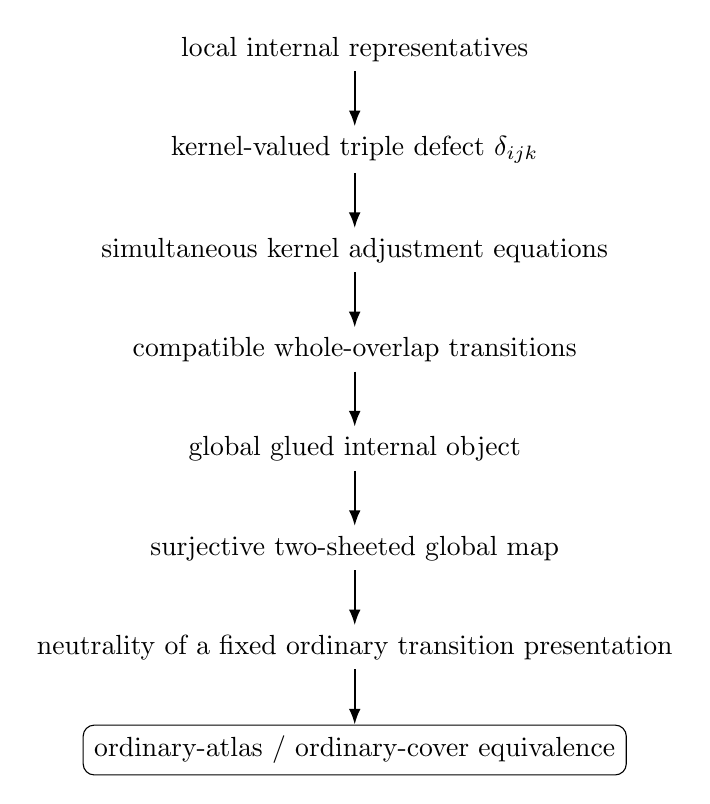
\begin{tikzpicture}[node distance=7mm, every node/.style={align=center}, arr/.style={-{Latex[length=2mm]},thick}]
\node (a) {local internal representatives};
\node[below=of a] (b) {kernel-valued triple defect $\delta_{ijk}$};
\node[below=of b] (c) {simultaneous kernel adjustment equations};
\node[below=of c] (d) {compatible whole-overlap transitions};
\node[below=of d] (e) {global glued internal object};
\node[below=of e] (f) {surjective two-sheeted global map};
\node[below=of f] (g) {neutrality of a fixed ordinary transition presentation};
\node[below=of g,draw,rounded corners,inner sep=4pt] (h) {ordinary-atlas / ordinary-cover equivalence};
\draw[arr] (a)--(b);\draw[arr] (b)--(c);\draw[arr] (c)--(d);\draw[arr] (d)--(e);\draw[arr] (e)--(f);\draw[arr] (f)--(g);\draw[arr] (g)--(h);
\end{tikzpicture}
\end{equation}

Every arrow above the last box has now either closed or been converted to an exact equivalence at the claimed level.  The unresolved issue is no longer ``can local lifts be chosen?'', ``can they descend?'', ``can they glue?'', or ``is the global map two-valued?''.  It is whether the resulting neutral/non-neutral state survives removal of ordinary atlas redundancy.

This is precisely what the top-to-bottom program is supposed to expose.  The large visible structure behaves like a compressed system of equations.  Solving one variable by substitution does not guarantee fundamentality; it may only reveal another derived variable one level below.

\section{The updated mathematical dependency DAG}\label{sec:dag}

It is useful to separate two arrows that were conflated by the formal Task-31 endpoint name.

For a fixed ordinary transition presentation $S$:
\begin{equation}\label{eq:fixed-dag}
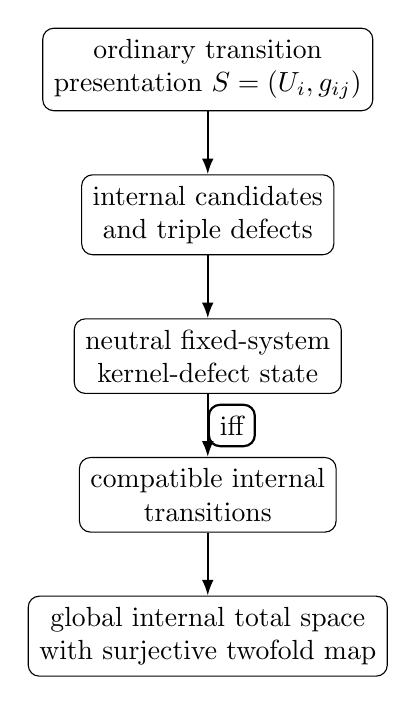
\begin{tikzpicture}[node distance=8mm, every node/.style={draw,rounded corners,align=center,inner sep=4pt}, arr/.style={-{Latex[length=2mm]},thick}]
\node (S) {ordinary transition\\presentation $S=(U_i,g_{ij})$};
\node[below=of S] (C) {internal candidates\\and triple defects};
\node[below=of C] (D) {neutral fixed-system\\kernel-defect state};
\node[below=of D] (L) {compatible internal\\transitions};
\node[below=of L] (I) {global internal total space\\with surjective twofold map};
\draw[arr] (S)--(C);\draw[arr] (C)--(D);\draw[arr] (D)--node[right]{iff}(L);\draw[arr] (L)--(I);
\end{tikzpicture}
\end{equation}
This graph is closed at Task-31 strength.

For the underlying geometry, however, one more incoming quotient is missing:
\begin{equation}\label{eq:geometry-dag}
\begin{aligned}
 \boxed{\text{metric-oriented frame family / intrinsic geometry}}
 &\longrightarrow \boxed{\text{ordinary atlas equivalence class}}\\
 &\longrightarrow \boxed{S=(U_i,g_{ij})}\longrightarrow\cdots
\end{aligned}
\end{equation}
The first two boxes have not yet been reconstructed as formal interfaces.  Until they are, non-neutrality of one $S$ is not automatically non-neutrality of the underlying family.

\section{Why the negative example is valuable rather than defective}\label{sec:value}

The presentation-sensitive negative example is not something to discard.  It is an unusually strong negative control because it separates two notions that would otherwise be easy to identify prematurely:
\begin{description}[leftmargin=8mm,style=nextline]
 \item[Direct fixed-atlas liftability.] Lift every $g_{ij}$ continuously on the chosen whole overlaps.
 \item[Intrinsic geometric liftability.] Existence of a global upstairs object after admissible changes or refinements of ordinary presentation.
\end{description}

Task~31 proves that the first notion can fail even for a globally trivial underlying rank-three family.  Therefore the two notions are not definitionally identical in the current reconstruction.

\begin{proposition}[Paper-level diagnostic]
Any future atlas-independent definition of spatial liftability must classify the bare constant family underlying \code{badFamily} as liftable, or else it is still sensitive to redundant ordinary frame-chart choices.
\end{proposition}

The reason is constructive: the global identity trivialization $T_0$ already supplies a presentation with only trivial transitions.  A future intrinsic theory that cannot recognize this would be stricter than global lift existence itself.

\section{What Task XXXII must quotient}\label{sec:xxxii-target}

Task~32 should therefore not start by searching for another exotic negative example.  It should first repair the level of the invariant.

At minimum, the next formal layer must distinguish and relate three kinds of freedom:
\begin{enumerate}[leftmargin=*]
 \item \textbf{internal kernel gauge:} $u_{ij}\mapsto\varepsilon_{ij}u_{ij}$, already reconstructed;
 \item \textbf{ordinary frame-chart gauge:} $g_{ij}\mapsto h_jg_{ij}h_i^{-1}$, not yet quotiented;
 \item \textbf{ordinary cover refinement/change:} replacement of the atlas by a finer or otherwise equivalent ordinary atlas, also not yet quotiented.
\end{enumerate}

The target should be a presentation relation broad enough that two atlases of the same underlying frame family become comparable, but narrow enough that no standard bundle/cohomology theory is imported as the answer.

A possible neutral interface name is
\[
 \operatorname{OrdinaryAtlasEquivalent}(A,A')
\]
or, if the underlying bare family is made primary,
\[
 \operatorname{IntrinsicFrameLiftable}(E).
\]
The exact name matters less than the dependency boundary: atlas data must become presentation data rather than geometry.

\section{A precise closure program for Task XXXII}\label{sec:xxxii-program}

The next task should be compact but decisive.  The following sequence is sufficient.

\subsection{Stage A: formalize ordinary atlas change}

Freeze a bare metric-oriented rank-three family and two admissible ordinary atlases on it.  Define the chart-comparison maps $h_i$ where both presentations are simultaneously available, and prove the induced transition transformation law corresponding to \cref{eq:gauge-transform}.  Do not assume the $h_i$ have global internal lifts.

\subsection{Stage B: realize the Task-31 good/bad pair as one underlying geometry}

Using the explicit constant family, prove formally that the trivial presentation and \code{badFamily}'s two-chart presentation belong to the same underlying family and are related by the new ordinary-atlas comparison.  This should become the first mandatory negative control:
\begin{equation}\label{eq:bad-repair}
 \text{same underlying family},\qquad
 S_{\mathrm{good}}\text{ neutral},\qquad
 S_{\mathrm{bad}}\text{ non-neutral}.
\end{equation}
Therefore the Task-31 fixed-system neutral predicate cannot itself be the final family-level invariant.

\subsection{Stage C: allow ordinary cover refinement}

Construct a notion of common ordinary refinement, not merely candidate refinement.  Transition functions and their local internal representatives must be restrictable along this refinement.  Prove exact composition/identity laws for repeated refinements and ensure that two atlas presentations of one bare family can be compared on a common refinement when the inherited topology permits it.

\subsection{Stage D: define atlas-independent liftability}

A natural first candidate is existential:
\begin{equation}\label{eq:familyliftable}
\begin{aligned}
 \operatorname{FamilyLiftable}(E)
 :\Longleftrightarrow{}&\ \text{there exists an admissible ordinary atlas of }E\\
 &\text{whose transition system is InternalLiftable}.
\end{aligned}
\end{equation}
But Task~32 should not accept \cref{eq:familyliftable} merely because it is easy.  It should prove that this predicate is invariant under the intended atlas-equivalence relation and, if possible, characterize it by an atlas-independent defect state.

\subsection{Stage E: descend the defect, not merely the Boolean answer}

The strongest target is an object
\[
 \Def(E)
\]
defined independently of a chosen ordinary atlas, such that
\begin{equation}\label{eq:intrinsic-defect}
 \boxed{
 \operatorname{FamilyLiftable}(E)
 \iff
 \Def(E)\text{ is neutral}.}
\end{equation}
If a complete quotient object is technically too large, Task~32 may first prove that \emph{neutrality} descends under atlas changes and ordinary cover refinements, mirroring the exact restraint used in Task~31 for candidate refinements.

\subsection{Stage F: only then search for a genuine negative geometry}

Once \cref{eq:intrinsic-defect} is available, ask whether there exists an underlying metric-oriented rank-three family with non-neutral atlas-independent defect.  The present \code{badFamily} is not such a witness because it is globally trivial.  A new negative example must survive all admissible atlas changes/refinements in the newly reconstructed sense.

No named characteristic class, standard non-spin bundle or cohomology theorem should be used to settle this.  The point is to discover whether the obstruction survives intrinsically from the reconstructed equations themselves.

\section{Possible Task-XXXII outcomes}\label{sec:outcomes}

There are three scientifically meaningful outcomes.

\paragraph{Outcome A: the obstruction disappears after ordinary presentation quotient.}
It may turn out that every inherited metric-oriented rank-three family becomes liftable after suitable ordinary refinement.  Then the Task-31 non-neutrality was entirely a fixed-atlas phenomenon.  This would be a positive geometric closure, but it must be proved, not inferred from the trivial control.

\paragraph{Outcome B: a genuine atlas-independent obstruction survives.}
Then Task~32 should construct or classify an underlying family whose defect remains non-neutral under every admissible ordinary atlas/refinement.  That would finally justify a geometric obstruction statement and would be the correct point for a late comparison with standard spin obstruction theory.

\paragraph{Outcome C: exact classification without a negative witness.}
Even if a non-neutral family-level example is too difficult, a theorem that family liftability is equivalent to neutrality of an atlas-independent reconstructed state would still close the conceptual dependency arrow.  The existence of non-neutral instances could then be separated into a later classification problem.

\begin{principle}[Patience is part of the proof boundary]
A reconstruction program should prefer one more exact quotient over an attractive but presentation-dependent conclusion.  Reaching a familiar diagram is not closure; closure occurs only when every arbitrary datum still present in the definitions has either been proved essential or quotiented as presentation.
\end{principle}

\section{Late conventional comparison: what may now be said, and no more}\label{sec:comparison}

Only after the intrinsic results are frozen is comparison with conventional language useful.  Earlier tasks reconstructed an internal group equivalent to the unit-quaternion/$SU(2)$ model, a visible group equivalent to $SO(3)$, and a two-element central kernel.  Part~XXX and Task~31 conditionally produce the familiar global shape of an equivariant twofold map over the oriented metric frame total space.  In standard spin geometry, atlas changes and cover refinements do not alter whether the underlying bundle admits a spin lift; the obstruction is attached to the bundle rather than to one arbitrary choice of local trivializations \cite{LawsonMichelsohn1989,Husemoller1994,Steenrod1951}.

This conventional fact is \emph{not} used to repair Task~31.  It serves only as a consistency diagnostic: our intrinsic reconstruction has not yet reached the conventional invariance boundary because ordinary atlas change has not yet been reconstructed in the Lean layer.

Likewise, the kernel-valued triple defect and its transformation law have the familiar shape of a degree-two lifting obstruction \cite{MilnorStasheff1974,LawsonMichelsohn1989}.  No formal identity with a Stiefel--Whitney class or any cohomology class is asserted.  Such a comparison is premature until the defect has first been shown to descend from transition presentation to underlying frame geometry.

\section{Formal decision table after review}\label{sec:decision}

\begin{longtable}{>{\raggedright\arraybackslash}p{0.52\textwidth}p{0.38\textwidth}}
\toprule
Question & Verdict after Task XXXI and source review\\
\midrule
\endfirsthead
\toprule Question & Verdict after Task XXXI and source review\\
\midrule
\endhead
$\Pi$ surjective onto all ordinary frames? & PROVED\\
Every ordinary frame has upstairs fibre? & PROVED\\
Every $\Pi$-fibre exactly a kernel torsor? & PROVED\\
Certified fibre cardinality exactly two? & PROVED\\
Local two-sheeted chart product? & PROVED\\
\code{IsCoveringMap Pi}? & NOT PACKAGED\\
Fixed-system liftability independent of internal representative choice? & PROVED\\
Fixed-system liftability independent of kernel gauge? & PROVED\\
Neutrality independent of Task-XXVIII candidate refinement? & PROVED\\
Full defect class canonical across candidates/refinements? & PARTIAL\\
Fixed ordinary system: liftable iff neutral? & PROVED\\
Universal fixed-presentation liftability? & REFUTED\\
Explicit neutral fixed presentation? & PROVED\\
Explicit non-neutral fixed presentation? & PROVED\\
Negative presentation realized by an inherited frame atlas? & PROVED\\
Underlying family of that negative atlas constant/global-trivial? & SOURCE-LEVEL PROVED BY DEFINITIONS; paper review consequence\\
Fixed-system neutrality invariant under ordinary atlas change? & NOT PROVED; explicit control strongly shows it cannot be assumed\\
Fixed-system neutrality invariant under ordinary cover refinement? & NOT PROVED\\
Atlas-independent family-level defect reconstructed? & NO\\
Atlas-independent non-liftable rank-three family exhibited? & NO\\
Conventional spatial Spin(3) identification? & DEFERRED\\
3+1 Lorentzian spin structure? & NO\\
Experiment 1 / Experiment 2 marriage? & NO\\
Physical spin or dynamics? & NO\\
\bottomrule
\end{longtable}

The key change relative to the Task-31 audit is not a retraction of any theorem.  It is a sharper statement of the object to which those theorems apply.

\section{Engineering provenance and failed builds}\label{sec:engineering}

Task~31 preserves five failed builds.  All are engineering failures rather than refutations of intended mathematical statements:
\begin{enumerate}[leftmargin=*]
 \item an ambiguous \code{OrdinaryTransitionSystem} name was resolved by namespace qualification;
 \item a rewrite in fibre transitivity used \code{mul_smul} in the wrong direction and was repaired without changing the statement;
 \item the quotient API spelling for an instance argument was unavailable and was replaced by \code{Quotient.eq_iff_equiv};
 \item an unused-binder warning in the defect-system structure was repaired by restating the field binder explicitly;
 \item the inherited overlap map required explicit family/index arguments during local-covering hardening.
\end{enumerate}

No intended theorem was weakened.  One expected-positive proposition, universal liftability, was not hidden when it failed: it is stated formally and its negation is proved by the explicit system.  This is exactly the desired failbuild/result provenance discipline.

\section{What Part XXXI has actually accomplished}\label{sec:accomplished}

The strongest theorem package that survives the review without qualification is substantial:

\begin{theorem}[Part-XXXI fixed-presentation closure, informal paper form]
Let $S$ be a fixed inherited ordinary transition system and $P:\Lift\to\Gvis$ the certified internal projection.  Then the following are equivalent:
\begin{enumerate}[leftmargin=*]
 \item compatible continuous internal transitions for $S$ exist;
 \item the Task-29 simultaneous kernel equations are solvable;
 \item the Task-31 global kernel-defect neutrality proposition for $S$ holds.
\end{enumerate}
Whenever they hold, the Task-30 gluing construction yields a global locally trivial internal total space with a continuous free fibrewise transitive right $\Lift$-action and a continuous surjective equivariant map onto the ordinary frame total space.  Every fibre of that map is exactly a kernel torsor and has two points for the certified kernel.  The local chart model is two-sheeted.
\end{theorem}

In addition, the space of fixed ordinary transition presentations contains both neutral/liftable and non-neutral/non-liftable examples.

What Part~XXXI does \emph{not} establish is that the neutral/non-neutral label is unchanged when the ordinary frame atlas itself is replaced by another admissible presentation of the same underlying family.

\section{The patience point: why stopping here would be premature}\label{sec:patience}

The last several tasks have repeatedly approached what looked like a final boundary.  Each time, formal closure at one level made the next lower dependency visible.  This is not wasted motion.  It is the central diagnostic value of the experiment.

At Part~XXIX the difficulty was a simultaneous kernel equation.  Part~XXX showed that solving it really would construct the global object.  Task~31 solved the logical existence classification for a fixed ordinary system and even supplied an explicit negative witness.  The source-level review then showed that this negative witness sits on a globally trivial underlying family and is created by a redundant global ordinary chart whose transition map itself has no global internal lift.

Thus the next question is not ``why did Task~31 fail?''  It did not fail.  The correct question is:
\begin{center}
\emph{Which variable in the fixed-system obstruction is still derived rather than fundamental?}
\end{center}
The answer is now visible: the ordinary atlas presentation itself.

\section{Outlook: Part XXXII -- Ordinary-atlas descent and the genuine geometric obstruction test}\label{sec:outlook}

Part~XXXII should therefore be titled neutrally along the following lines:

\begin{center}
\textbf{Task XXXII -- Ordinary Atlas Change, Cover Refinement, and Atlas-Independent Internal Liftability: Descent of the Kernel Defect to the Underlying Frame Geometry.}
\end{center}

Its three hard targets should be:

\paragraph{Hard target A: ordinary-presentation equivalence.}
Formalize changes and refinements of the ordinary frame atlas on one underlying metric-oriented rank-three family.  Prove the induced law for $g_{ij}$ and common-refinement coherence.  Use the Task-31 good/bad pair as the mandatory control proving that direct fixed-atlas liftability is not the final invariant.

\paragraph{Hard target B: atlas-independent neutrality/liftability.}
Construct the weakest correct family-level predicate, and preferably an atlas-independent defect state, whose neutrality is equivalent to existence of a global internal lift after admissible ordinary presentation changes.  Prove independence from ordinary chart gauge and ordinary cover refinement rather than assuming it.

\paragraph{Hard target C: genuine obstruction decision.}
After the atlas quotient is closed, decide whether non-neutral underlying families actually exist in the inherited class.  A positive universal theorem, a genuine atlas-independent negative example, or an exact necessary-and-sufficient classification would all be valid closure outcomes.  Do not import standard spin obstruction theory to force the result.

The stopping rule should be strict: if the family-level invariant is obtained, stop before the Experiment-1/Experiment-2 marriage.  Only then will it be legitimate to ask whether the resulting spatial lift is the same deeper structure seen from the independently decomposed split-complex Lorentz branch.

\section{Conclusion}\label{sec:conclusion}

Task~31 looked capable of ending the spatial reconstruction.  Instead it produced a more valuable result.  It closes the fixed-transition-system lifting problem exactly: neutrality of the reconstructed kernel-defect state is equivalent to compatible internal transitions, and neutrality produces the fully global, surjective, equivariant, two-sheeted internal object anticipated by Parts~XXIX--XXX.  Universal fixed-presentation liftability is genuinely false, and the Lean development exhibits both neutral and non-neutral systems without importing characteristic classes, cohomology or a standard non-spin example.

But the negative example itself exposes the next layer.  Its underlying rank-three metric-oriented family is constant and globally trivialized by the very source that constructs the non-liftable two-chart presentation.  The non-neutrality therefore belongs, at the present theorem boundary, to the chosen ordinary transition presentation.  Task~31 has removed internal representative dependence but has not yet removed ordinary atlas dependence.

The Conservation of Difficulty has therefore not ended; it has sharpened.  What appeared to be the final global kernel obstruction has split into two levels:
\[
 \text{fixed-presentation defect}
 \qquad\text{and}\qquad
 \text{still-unreconstructed atlas-independent geometric defect}.
\]
The first is now exact.  The second is the target of Part~XXXII.

There is no reason to rush the final identification.  The purpose of the top-to-bottom program is precisely to refuse a familiar name until the dependency system has been expanded far enough that arbitrary presentation variables have disappeared.  Task~31 has taken another substantial step downward.  It has not reached the basement.  Part~XXXII must test whether the obstruction survives when the ordinary atlas itself is finally treated as presentation rather than substance.

\printbibliography

\end{document}
